\chapter{Experiments}

In this chapter we describe how we implemented the chosen song encoding methods, retrieved representations for each song in our 16594 songs dataset, calculated distances between all the songs and evaluated each methods based on the playlists from our user dataset. We also describe the evaluation method we chose and propose what we expected. As it is the same for all our implemented methods we will start with the last two mentioned. 
\section{Expectations}

Before we introduce any results we summarize what we expected. Even before reading any literature, we made two main predictions. 
\begin{itemize}
    \item \textbf{First:} Audio-based methods will perform better than text-based methods.
    \item \textbf{Second:} More advanced methods will outperform simpler machine learning methods.
\end{itemize}
These were based on our intuition and later also supported by reading into this topic, where most of the papers we studied were describing neural networks performing similar audio or text-based recommendation or classification and their results were compared to simpler algorithms. However, this has not proven to be accurate with our evaluation dataset. The reasons for why it might be the case are described at the end of this chapter in the \textbf{Discussion} section. \\
We were also hoping, that the text-based methods will not be complete irrelevant. In this case, we were right, but only to the extend that the text-based methods are not irrelevant in comparison to the audio-based methods. Overall, all the methods have shown that they seem to lack the properties to be useful as methods for recommendation.
\section{Evaluation}

\subsection{Wanted recommender-system features}
We already touched this in the introduction but it is useful to revise what we want from a good recommendation system and what its most important features are. Let's skip the software part for now (as it will be discussed further in the \textbf{Web application} chapter and focus purely on what it recommends. Probably the most crucial property a recommendation system should have is that it should include the items the user actually likes between the first 10 to maybe 50 recommendations. Because it does not really matter if an item the user would like ends up on the 500th or 5000th position. People rarely go that deep. \\
Another thing we would want is for the system to be able to improve its recommendations with a rising amount of data it acquires about a user. In our case this means, that we would expect the predictions to be better for users with longer playlists. \\
Even though the whole idea of this thesis is to approach recommendation more loosely, we still want our methods to posses these features to at least some reasonable extend. Also, as these are the properties other recommendation systems are being evaluated on, we can gain a better understanding of the features our methods share with other recommendation techniques as well as their where they differ. 
\subsection{Evaluation measures}
To test the wanted features described in the section above we performed evaluation as follows. \\
Our dataset contains 45045 playlists that can be used to evaluate our algorithms. For each method, we did a 5-cross-validation where in validation epoch, every playlists $p_i$ was divided into two parts a training part $p_{i_{train}}$ and a testing part $p_{i_{test}}$ with an approximately 80:20 ratio. A higher priority was set on the fact that the test part always had to contain at least one entry (meaning that for playlists of length 2, the ratio was 50:50). \\
Afterwards for each song $ s_k $ from our song dataset $S$, the similarity of the whole $p_{i_{train}}$ to $s_k$ which we denote as $ sim(p_i, s_k) $ was calculated as $sim(p_i, s_k) =$ $\sum_{s_j\in{p_i{_{train}}}} cos_sim(s_i, s_j) $ where $ i \neq j$ and $cos_sim$ is the cosine similarity as defined by Python scikit-learn package. These similarities were then sorted and it was determined at what position the songs from $p_{i_{test}} $ that actually belong to the playlist came. \\
These positions were then used to calculate multiple evaluation measures used to assess how well does each algorithm predict the missing part of a users playlist. For this we chose the following for methods:
\begin{itemize}
    \item Recall at 10 (= \textbf{R@10}) defined as the number of songs from $p_{i_{test}} $ that placed in the top ten most similar songs.
    \item Recall at 50 (= \textbf{R@50}) defined as the number of songs from $p_{i_{test}} $ that placed in the top fifty most similar songs.
    \item Recall at 100 ( = \textbf{R@100} ) defined as the number of songs from $p_{i_{test}} $ that placed in the top hundred most similar songs.
    \item Normalized cumulative discounted gain (= \textbf{nCDG}) defined as 
    $${nDCG_{r}} = \frac{DCG_{r}}{IDCG{r}} $$
    where 
    $${DCG_{r}} =\sum_{i=1}^{r}{\frac {rel_{i}}{\log _{2}(i+1)}} $$ 
    is the discounted cumulative gain at position r and 
    $$ {IDCG_{r}} =\sum _{i=1}^{|REL|}{\frac {2^{rel_{i}}-1}{\log _{2}(i+1)}} $$
    is the ideal discounted cumulative gain at r
    where $r$ is in our case the number of songs that had to be predicted, the $rel_i$, meaning relevance, is the same for all songs as all songs in one playlists have the same relevance and $|REL|$ is the list of relevant items (in our case the songs from $p_{test}$).
    \item Average rank of a song from the $p_{i_{test}}$ set $ \boldsymbol{ (= \overline{rank})} $ which we included after the first four mentioned did not really meet our expectations.
    \item The distribution of rankings of songs from the test part of each playlists. Meaning that we summed the number of occurrences of a song from $p_test$ on each individual position from 1 to 16594 and divided it by the number of all songs that were in a testing part of some playlist. 
    
\end{itemize}
We calculated for each of these measures for each playlist and then averaged over the whole playlist dataset. 
\section{Text method experiments}

\subsection{TF-idf experiments}\label{ssec:TF_idf}


\subsubsection{Input}
The lyrics for each song were stripped of all punctuation characters as well as apostrophes, converted into a single string. 
\subsubsection{Training}
Each lyric-string was appended to the whole training dataset which was then passed to an instance of \texttt{sklearn.feature\_extraction.text.TFidfVectorizer} where the method \texttt{fit\_transform} was called. The results were saved into a numpy file containing a sparse matrix. And the model was saved using pickle.\\

\subsubsection{Output}
The song representation were vectors of length 40165 which is the number of different words our dataset contained.

\subsubsection{Results}

The results of the TF-idf method were poor overall when it comes to satisfying the properties of recommender systems.In comparison to our other methods however, they placed well above average. \\

\begin{table}[h!]
\centering
\renewcommand{\arraystretch}{1.5}
\begin{tabu} to 1\textwidth {| c || X[c] | X[c] | X[c] | X[c] | X[c] | }
 \hline
 \textbf{method} & \textbf{R@10} & \textbf{R@50} & \textbf{R@100} & \textbf{nGDC} & $ \boldsymbol{\overline{rank}} $ \\
 \hline
 \hline
 Tf-idf & 0.04293 & 0.05051 & 0.05619 & 0.03594 & 7553 \\
 \hline
 PCA on Tf-idf & 0.05091 & 0.05909 & 0.06393 & 0.04107 & 7345 \\
 \hline
\end{tabu} \\
\caption{Table summarizing average TF-idf and Tf-idf with PCA values averaged over the 5 cross validation that were performed}
\label{table:1}
\end{table}

When looking at the number in \ref{table:1} we can see that only 4.3\% of songs that were in our $p_{test}$ sets ranked in the first ten, 5\% in the first fifty and 5.6\% in the first hundred. The average rank of a song from our $p_{test}$ was 7553 which is quite close to the middle. This does not really satisfy our goals that we set to achieve in recommender systems. We also crated a graph of the distribution of ranks (as we did for every method). The x-scale was scaled logarithmically as we are much more interested in what is going on between the first hundred songs than what is going on in the middle or at the end. And as one can see in \ref{fig:tf_idf_distribution}, it appears that according to the distribution, a song is more likely to end up in the first 10-100 songs than it is at the end. One could claim that this distribution is not random and favors ranks at the beginning, however not as strongly as we would want.\\
Another thing to notice in \ref{fig:tf_idf_distribution} is that there is a general trend for the Tf-idf method to perform worse on playlists with a greater length. This is the complete opposite of what we desire. One can see, that for playlists with length from 4 to 6, the ranks predicted for the missing songs were more likely to be higher than for playlists of length 21 and longer. The pink bar shows the overall distribution over 5000 bins over the dataset. 

\begin{figure}[h]
\centering
\begin{minipage}{.5\textwidth}
  \centering
  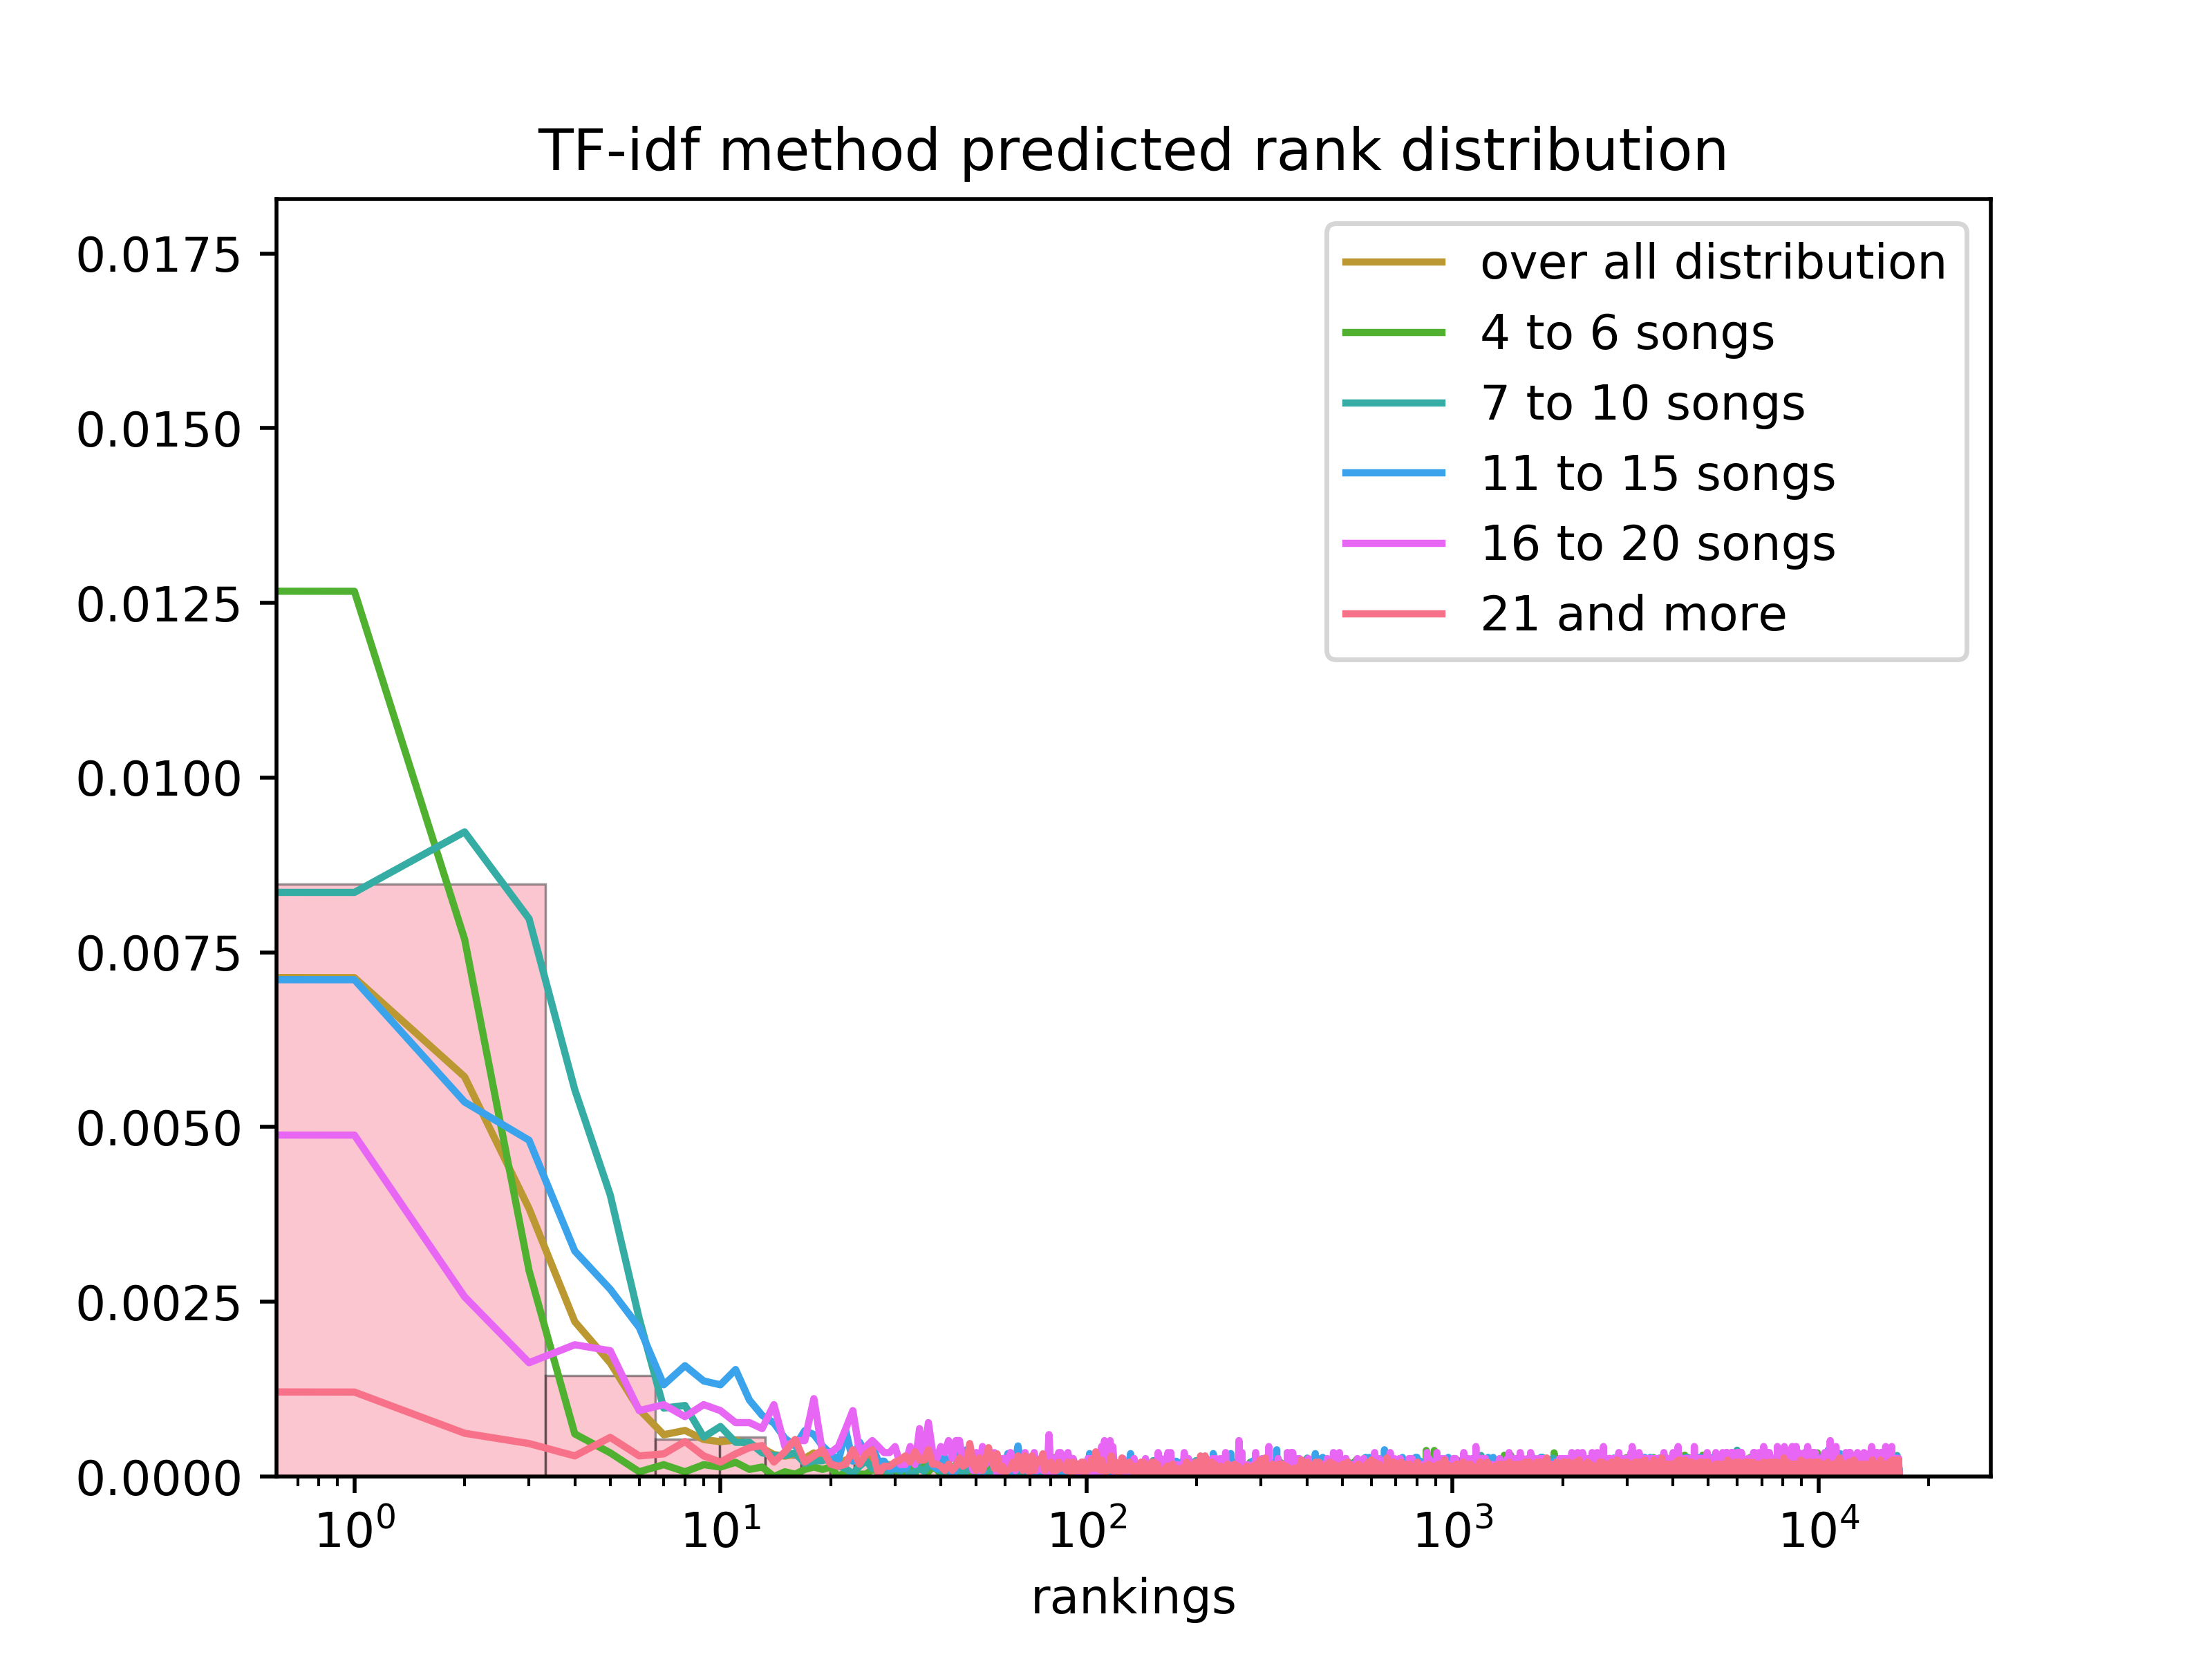
\includegraphics[width=1\linewidth]{./img/tf_idf_graph.png}
  \captionof{Distribution of ranks of songs from the $p_{test}$ set the tf-idf method assigned them.}
  \label{fig:tf_idf_distribution}
\end{minipage}%
\begin{minipage}{.5\textwidth}
  \centering
  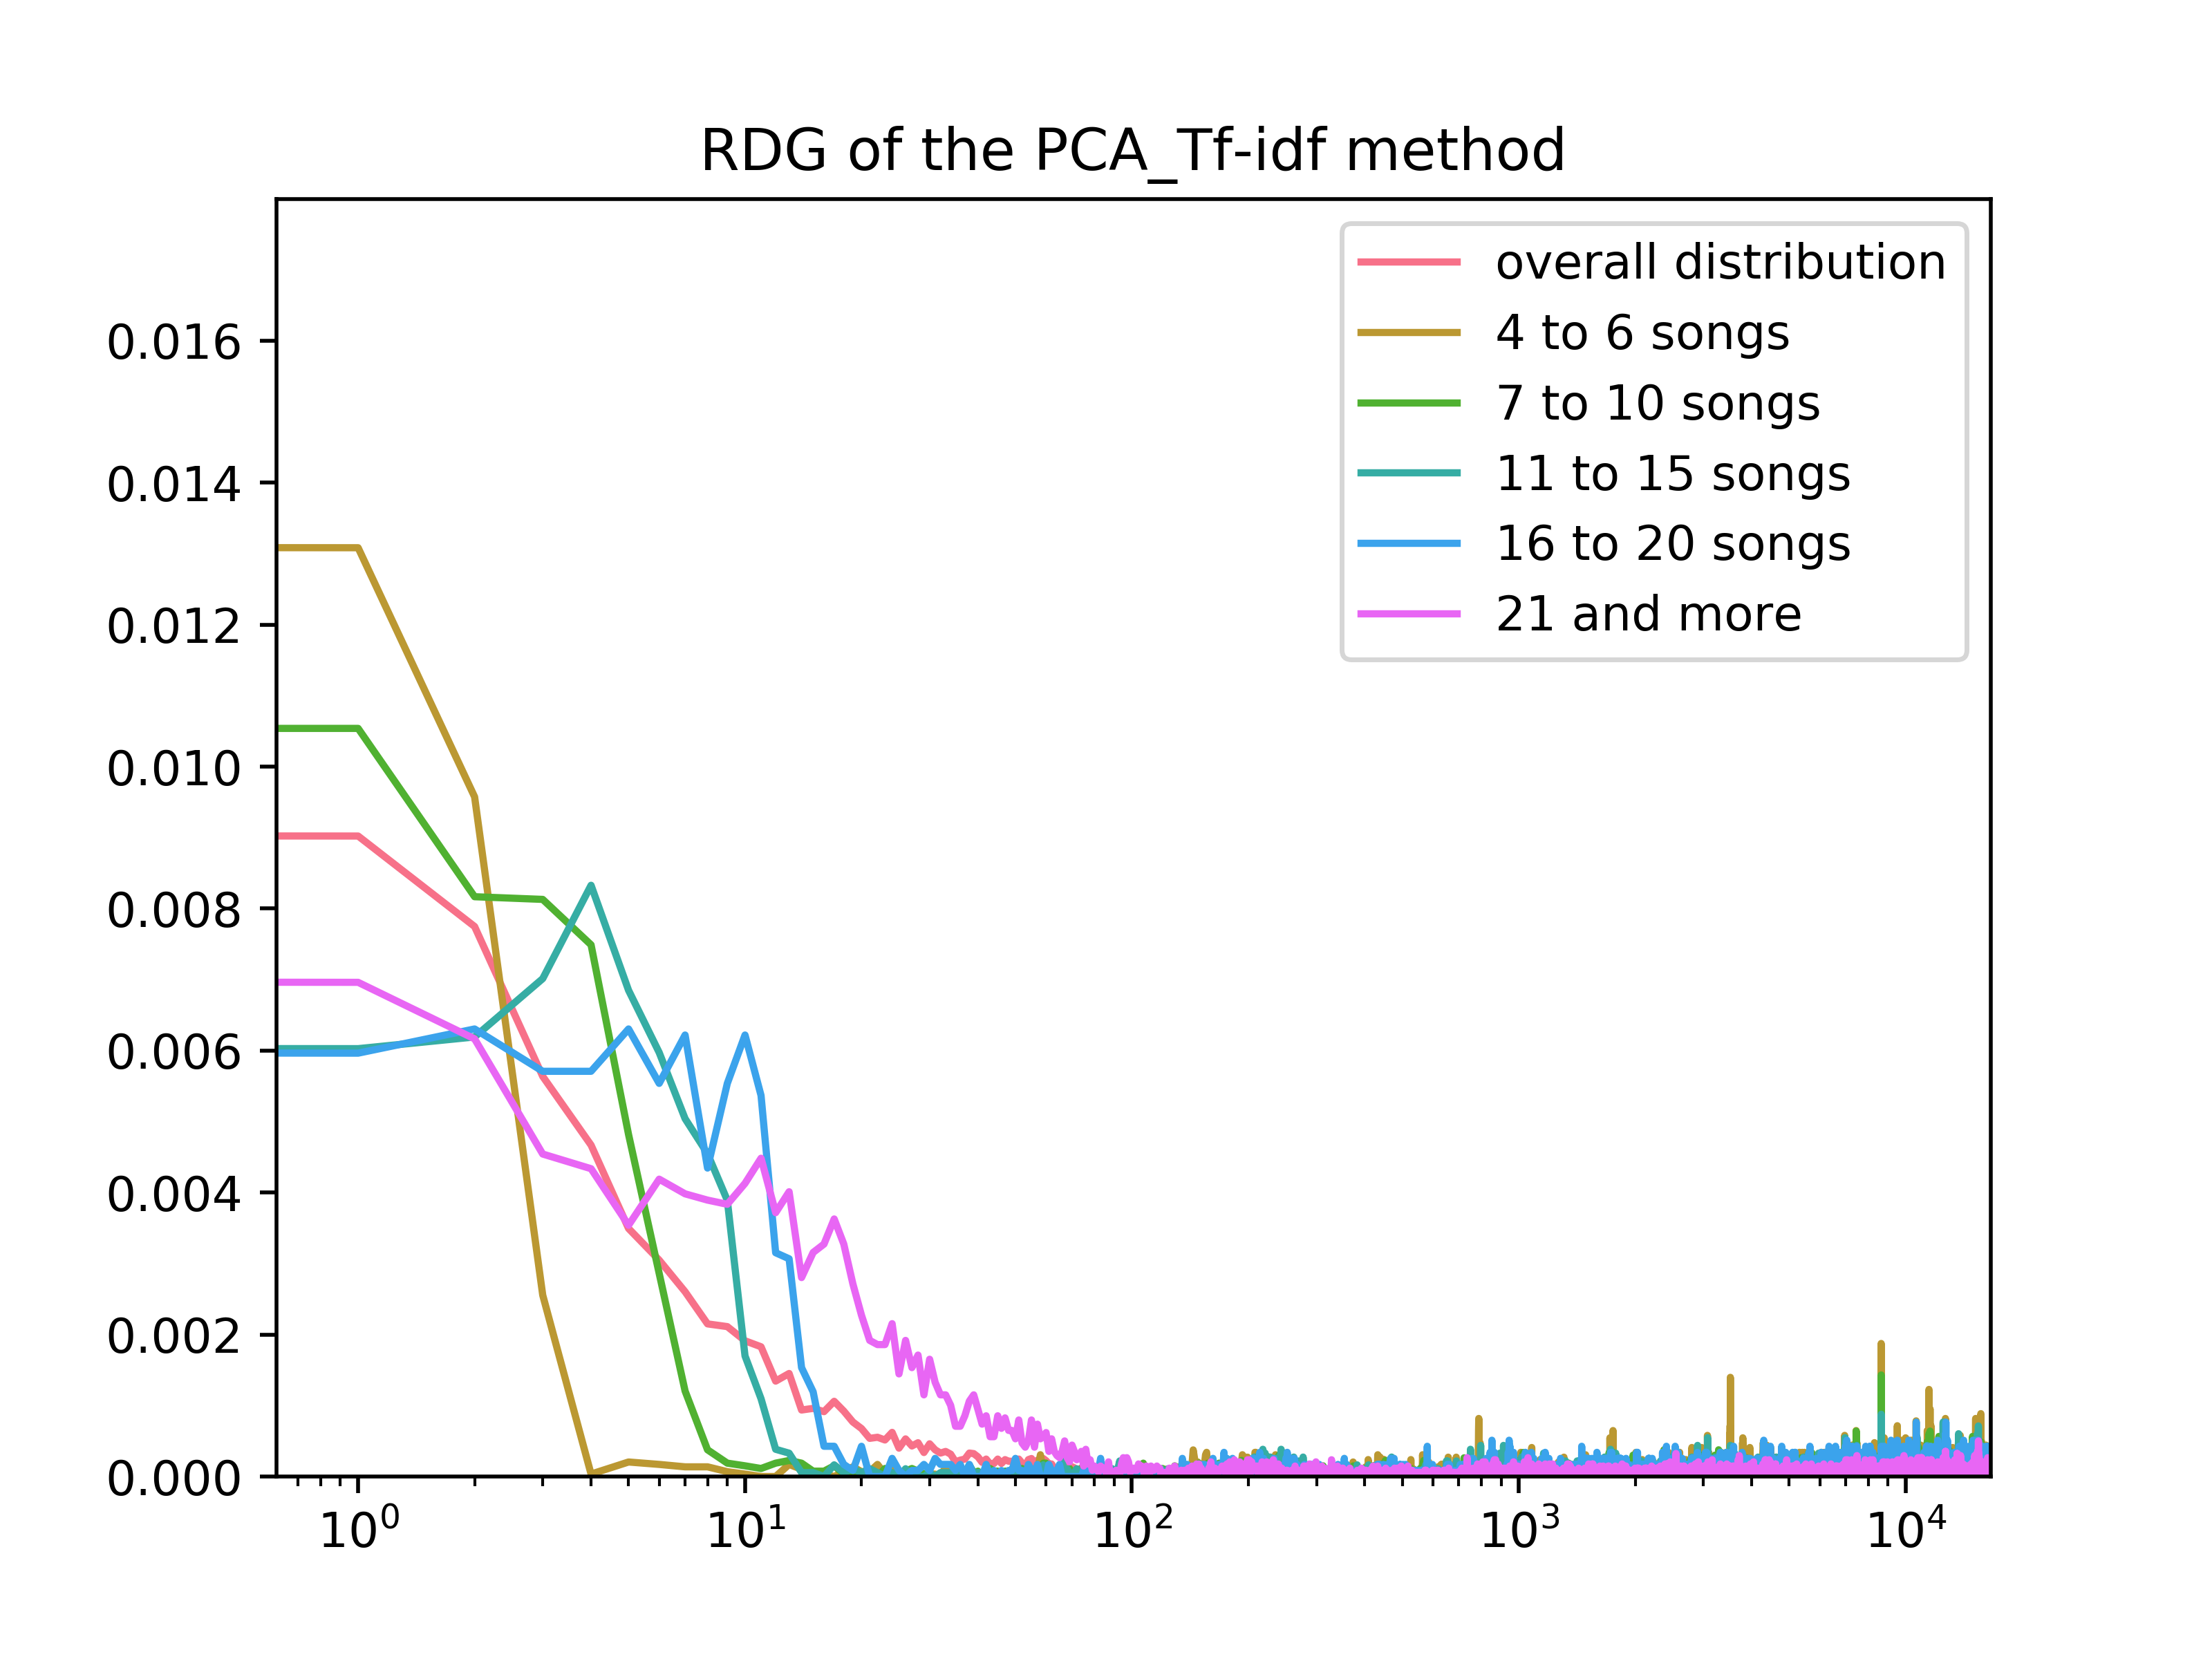
\includegraphics[width=1\linewidth]{./img/pca_tf_idf_graph.png}
  \captionof{Distribution of ranks of songs from the $p_{test}$ for tf-idf vectors as input into PCA}
  \label{fig:pca_tf_idf_distribution}
\end{minipage}
\end{figure}
\subsection{PCA on Tf-idf}\label{ssec:PCA_on_tf_idf}

Because Tf-idf has proven to yield good results we want to implement it. The long vectors pose a problem to our web application though, as it is necessary to calculate the distance between a newly added song and all the songs that are already in the database. Since the machine on which our application is running does not have such computational power as those we run our evaluations on, we decided to try to reduce the dimensions using PCA because has proven quite effective with mel spectrograms.

\subsubsection{Input}
As input, we provided the tf-idf vectors which we acquired as described \ref{ssec:TF_idf}. We did not normalize them.

\subsubsection{Training}
For training we first run a PCA from Python's \texttt{sklearn.decomposition.PCA}. We then chose the space were the explained variance ratio was equal to 90\% which left us with 4457 features. This means, our Tf-idf vector went from 40165 to 4457 dimensions. 

\subsubsection{Output}
The output were vectors of length 4457.

\subsubsection{Results}
The results of the PCA-reduced Tf-idf vector turned out to be better then those of full length. As we can see in \ref{table:1} 

\subsection{Word2Vec experiments}\label{ssec:w2v_experiments}

\subsubsection{Input}
The input for our W2V model was the same as for the Tf-idf method.

\subsubsection{Training}
In the case of Word2Vec, we did not perform any training. Instead, we used a pre-trained W2V model from Google (the first 200000 words which covered all the words in our lyric dataset). If there was a word in a song that is not in our subset added in the web application, would be ignored.

\subsubsectio{Output}
The output for a document of the Google model is a vector of fixed length 300. This is significantly lower than the Tf-idf vector.

\subsubsectio{Results}
The small size of the vectors being produced by the W2V method are a significant advantage of this method. However the results it yielded make it below average even compared to our other methods.

\begin{table}[h!]
\centering
\renewcommand{\arraystretch}{1.5}
\begin{tabu} to 1\textwidth { | c || X[c] | X[c] | X[c] | X[c] | X[c] |}
 \hline
 \textbf{method} & \textbf{R@10} & \textbf{R@50} & \textbf{R@100} & \textbf{nGDC} & $ \boldsymbol{\overline{rank}} $ \\
 \hline
 \hline
 W2V & 0.00768 & 0.01354 & 0.01983 & 0.00909 & 7682 \\
 \hline
\end{tabu} \\
\caption{Table summarizing average W2V values averaged over the 5 cross validation that were performed}
\label{table:2}
\end{table}

The table shows much lower numbers than for the Tf-idf method. Only 0.7\% of songs from the $ p_{test} $ set ranked in the top 10, 1.3\% in top 50 and 2.0\% in top 100. The average rank was 7682. That does not seem to be as bad compared to Tf-idf so it suggests that the songs did not place at the last ranks, but also not at the first ranks. \\
When looking at the distribution graph, it is very clear that the gap here between the accuracy of predicted ranks for short and longer playlists is huge. Although not great, it performs much better for short playlists. For playlists as short as 7, the performance drops significantly and it appears that for playlists with length 11 and more, the trend is opposite than what we would want, meaning, that it is more likely that a song from the $p_{test}$ set does ranks between the last 1000 than between the first 1000 if the rank is predicted based on a playlists of length at least 11.

\begin{figure}[h]
    \centering
	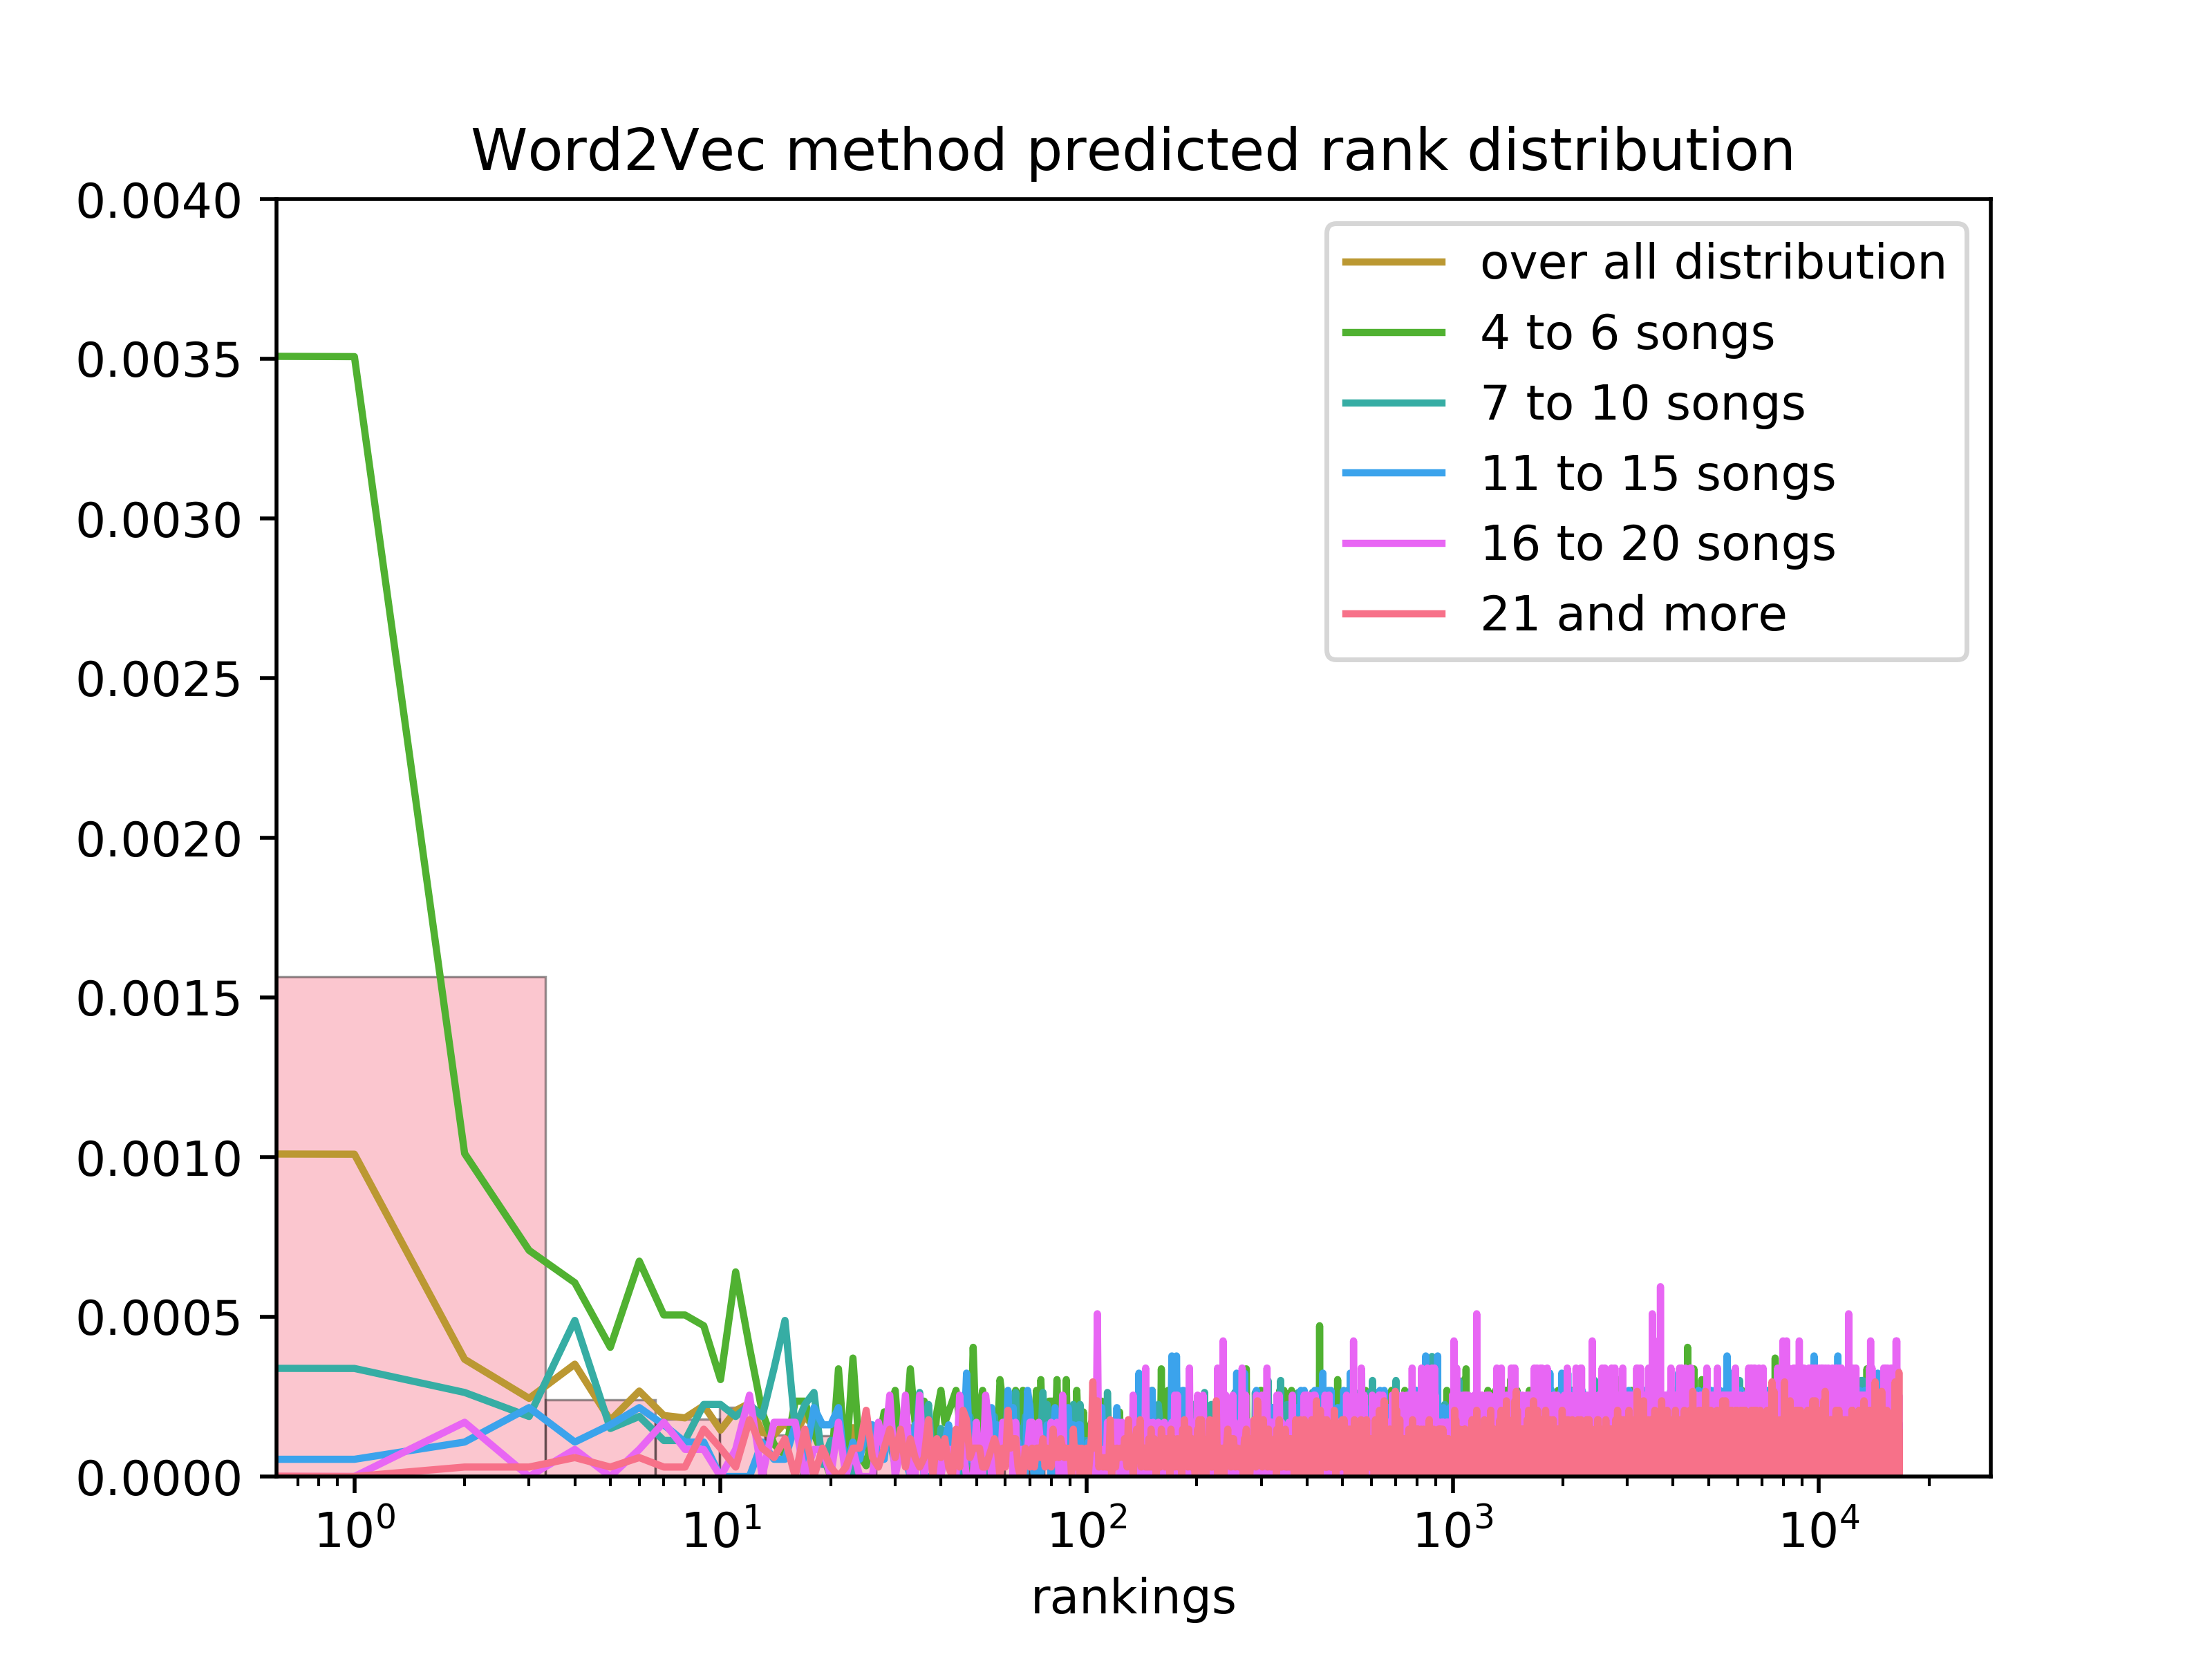
\includegraphics[width=120mm]{./img/w2v_graph.png}
	\caption{Distribution of ranks of songs from the test set the w2v method assigned them.}
	\label{fig:w2v_distribution}
\end{figure}

\subsection{SOM experiments}
We used a python library called \texttt{minisom} \cite{Vettigli2019}
\subsubsection{Input}
We chose the W2V vectors from \ref{ssec:w2v_experiments} as input for our self organizing map, mainly because of their length and also because we were hoping, that the SOM could improve its results.

\subsubsection{Training}
We build a self organizing map with a grid size 5 times our dataset size (16594) and the number of iterations was also 5 times our dataset size. We saved a model after each multiple of 16594 iterations and interestingly, the representations did not change after 33 187 iterations (meaning 2*16594). It was also necessary to normalize our input vectors and set learning rate to 0.2. Otherwise the songs formed 3 to 5 large clusters on the grid placing thousands of songs on the same coordinate. 
\subsubsection{Output}
The output representation for each song was a vector of length two. The whole dataset then could be displayed on a 2D map. 
When we then tried to display the map with all the songs, the size of the image would have to be immense so that all 16594 songs would be recognizable. The problem was that there were many songs to display on the map and the titles overlapped. Because of that, we decided to randomly select 20 playlists and show where the different songs that belong to each playlist placed on the map. Each playlist has its own color. This map is depicted in \ref{fig:som_map}. Obviously, the playlists do not really form any visible clusters.
\begin{figure}[h]
    \centering
	\includegraphics[width=140mm]{./img/som_map.png}
	\caption{The location of different songs from 20 randomly selected playlists on the map created by SOM. Each playlist has its own colour.}
	\label{fig:som_map}
\end{figure}
\subsubsection{Results}
The fact that the playlists do not form clusters is also supported by the fact that the overall results for the self organizing map algorithm are quite poor. Actually it is the worse method that we implemented and our hope to improve the results of W2V were not fulfilled.

\begin{table}[h!]
\centering
\renewcommand{\arraystretch}{1.5}
\begin{tabu} to 1\textwidth { | c || X[c] | X[c] | X[c] | X[c] | X[c] |}
 \hline
 \textbf{method} & \textbf{R@10} & \textbf{R@50} & \textbf{R@100} & \textbf{nGDC} & $ \boldsymbol{\overline{rank}} $ \\
 \hline
 \hline
 SOM with W2V & 0.00084 & 0.0038 & 0.00664 & 0.00192 & 8152 \\
 \hline
\end{tabu} \\
\caption{Table summarizing average SOM values averaged over the 5 cross validations}
\label{table:som}
\end{table}

The distribution graph of the SOM method clearly shows, that the distribution of ranks is random or worse which is also suggested by the fact that the average rank is 8152 which almost in the middle of 16594. The main reason for the failure of this method is unclear but it is possible that the data from the W2V vectors that already contains too little information for the SOM network to be able to cluster data based on it. Another possibility could be, that even if the input vectors were longer or contained more information, the SOM network would not be able to provide satisfying results because two dimensions are simply too little to represent the complexity of 
\begin{figure}[h]
    \centering
	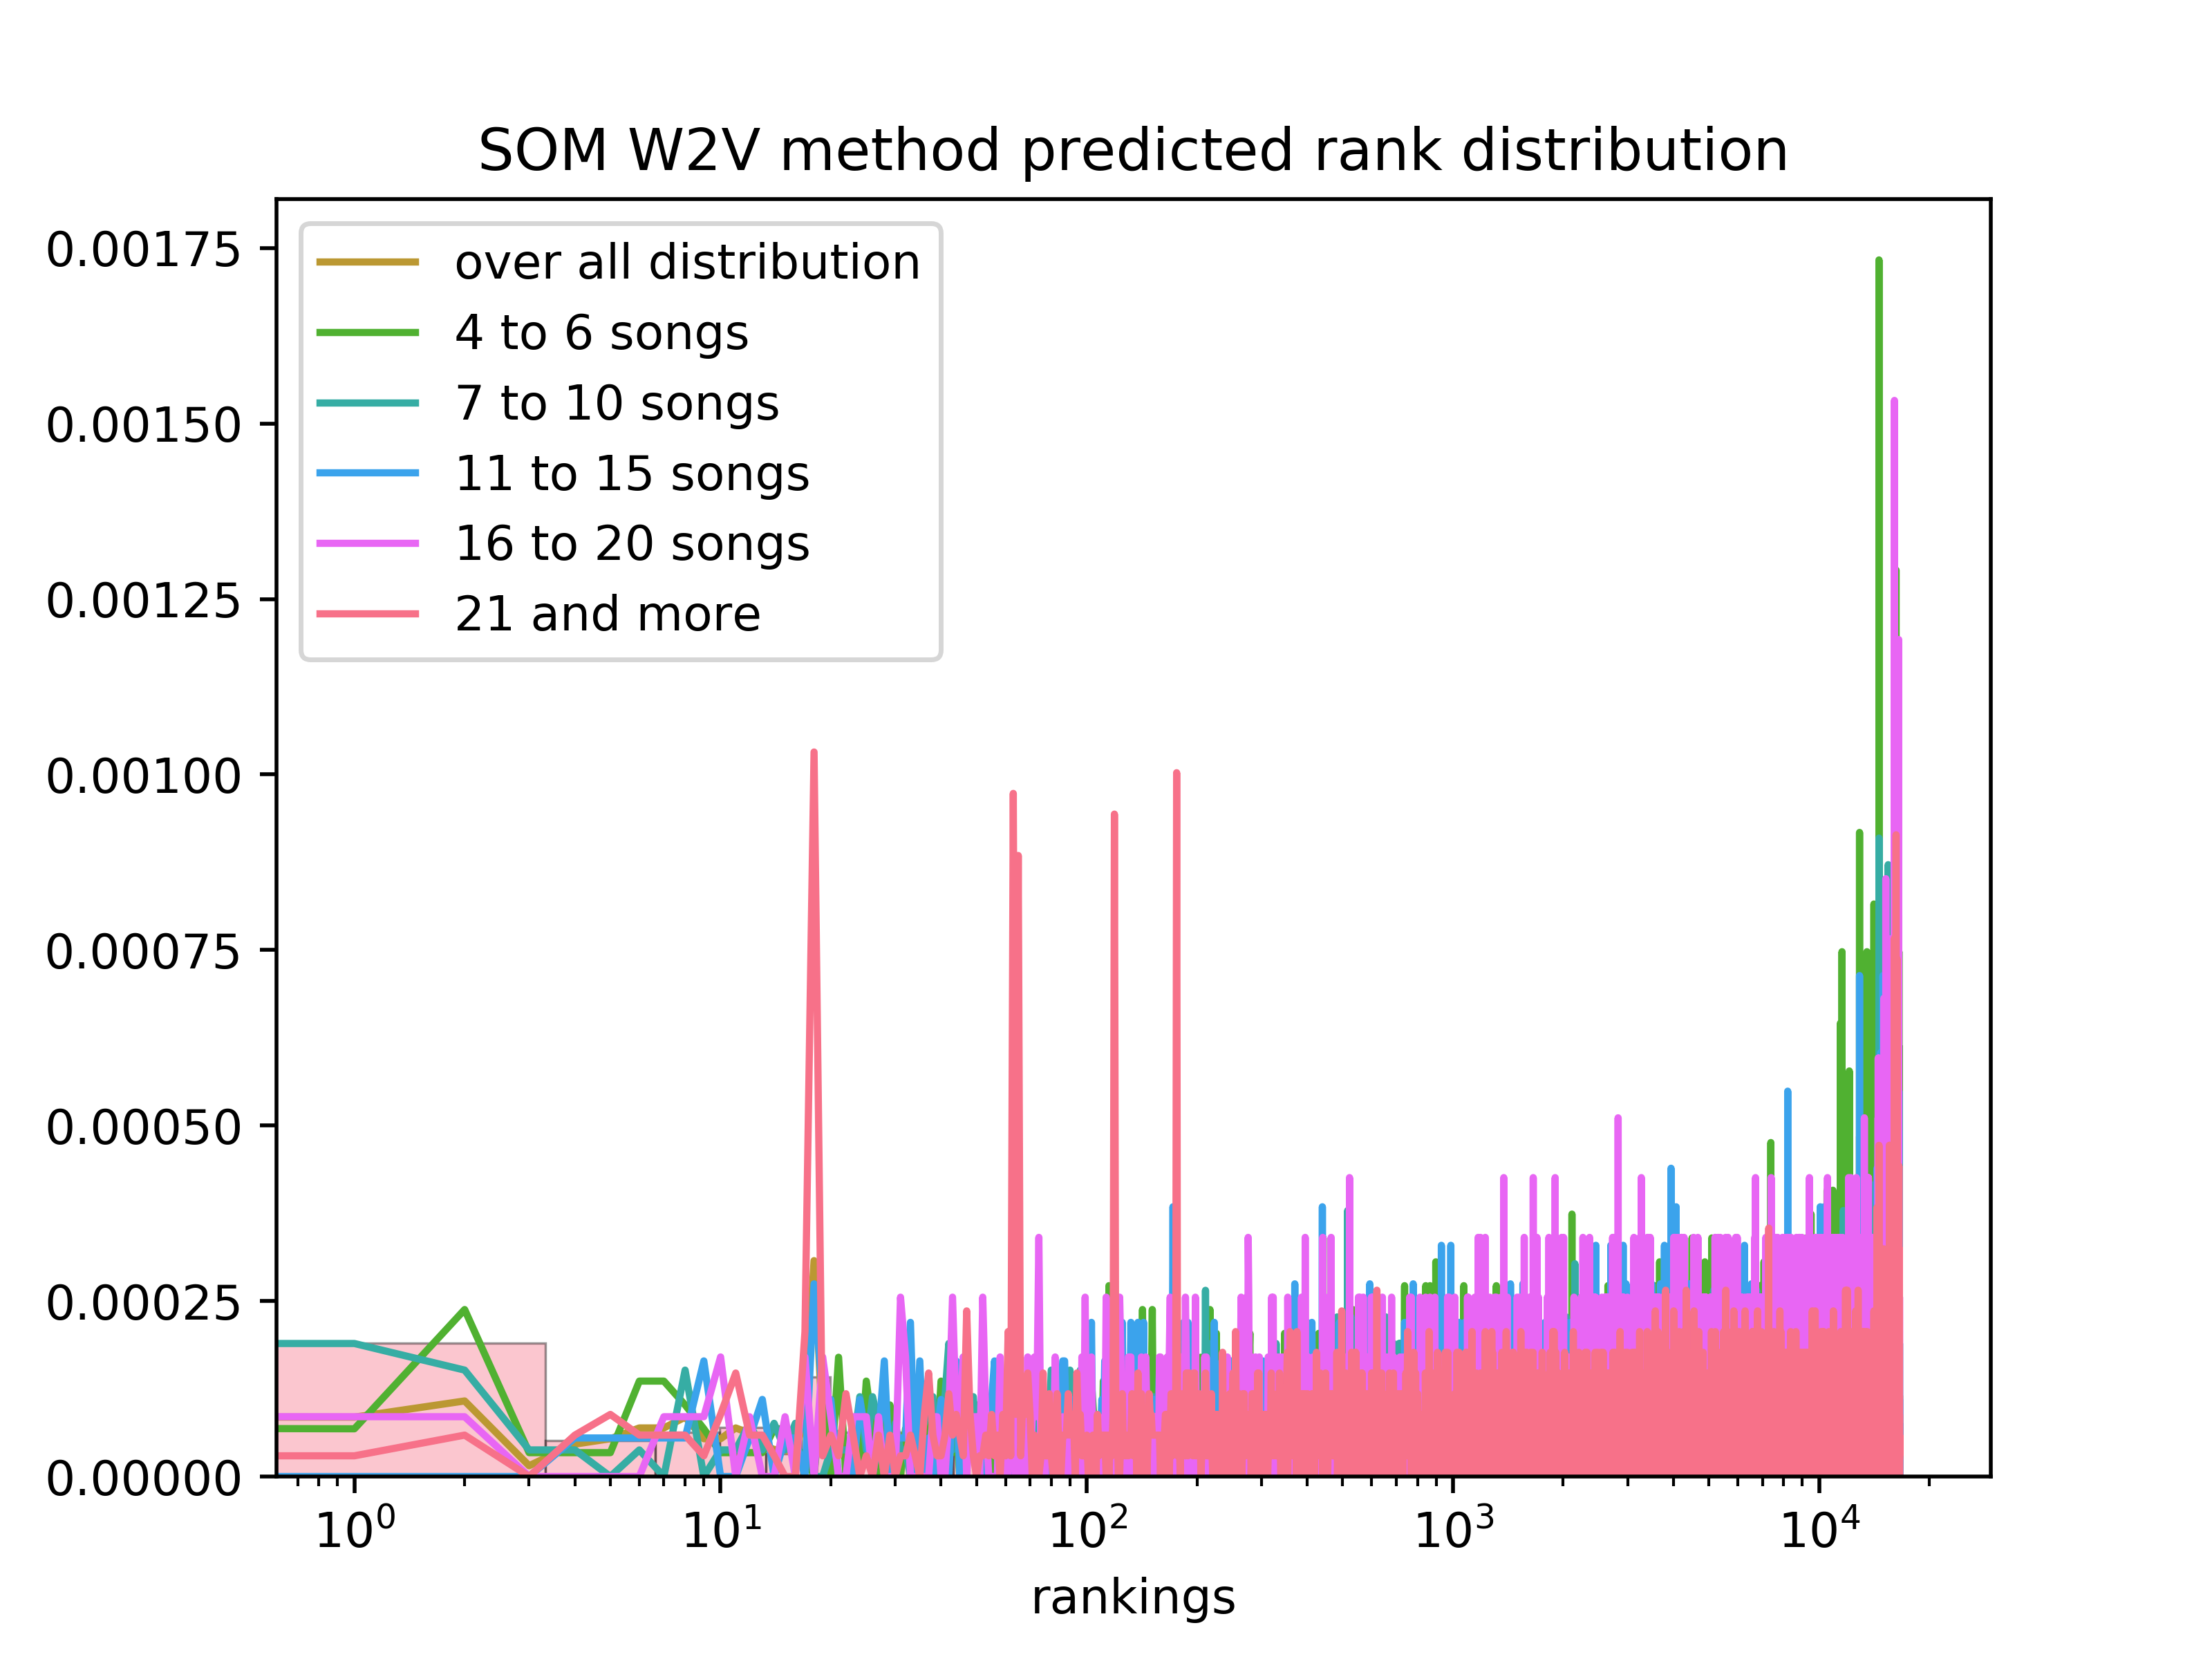
\includegraphics[width=120mm]{./img/som_w2v_graph.png}
	\caption{Distribution of ranks of songs from the test set the SOM method assigned them.}
	\label{fig:som_distribution}
\end{figure}
\section{Audio method experiments}
\subsection{Audio preparation}\label{ssec:audio_prep}

In order to encode audios of songs, we first needed to acquire some form of the music to become our standard. To make our audio information suitable for machine learning, we decided to extract audios of the same length so our vectors (spectrograms, mel-spectrograms and mfccs are also of the same length). Since all songs have different lengths and also, one complete 3.5 minute long song results in a spectrogram of size 5214x2206 which when flattened is a vector of length 11 502 084. Therefore we decided to extract 15 second excerpts from each song to create spectrograms, mel-spectrograms and MFCCs from those. We took 5 seconds between the 15th and 20th second, 5 seconds starting in the middle of the song and 5 second starting 15 seconds before the end. We did not start at the beginning and the end because in some songs, there is silence or applause or some talking before the actual song starts. \\

It was also necessary to decide on some parameters for spectrograms, mel-spectrograms and MFCCs. As stated previously, our neural networks were inspired by \cite{inproceedings_RNNs} where they also performed parameter optimisation. We decided to use their parameters as input for all our methods. It is possible that some parameters values suite some methods better than others but because of the amount of methods we tested we decided it would too difficult to optimise them for each method. We also think, that it a good idea to have all methods work with more or less the same input as their comparison is less ambiguous. \\
The resulting choices were following. We set window width $w$ to 0.2 and window overlap $w_o$ to 0.5$w$ = 0.1. For mel-spectrograms it is also necessary to choose Mel frequency bands which was set to 320 as for values above 320, the performance of neural networks did not increase. For MFCC coefficients we decided to set the number of MFCC coefficients to 320 which is the same as the number of Mel frequency bands.

We used Python's \texttt{librosa} library \cite{brian_mcfee_2019_2564164} to cut our songs and to generate our spectrograms, mel spectrograms and MFCCS using functions \texttt{librosa.core.stft} for spectrograms \texttt{librosa.feature.mel_spectrogram} for mel-spectrograms and \texttt{librosa.feature.mfcc} for MFC coeficients. The audio data for training was stored in .wav files.

\subsection{Raw Mel spectrograms}\label{ssec:raw_mels}
The input for mel spectrograms was the 15 second long audio described in \ref{ssec:audio_prep}. Extracting spectrograms does not require any training. It a is mathematical procedure explained in \ref{ssec:mel_spectrograms_intro}.

The mel-spectrograms we got after transforming a 15 second long audio with 320 Mel frequencies bands was a matrix of size 408x320 which when flattened is a vector of size 130560. This turned out to be too long to implement in our application, however because we did not realize that at first, we tested this method and got the following results.

\subsubsectio{Results}
\begin{table}[h!]
\centering
\renewcommand{\arraystretch}{1.5}
\begin{tabu} to 1\textwidth { | c || X[c] | X[c] | X[c] | X[c] | X[c] |}
 \hline
 \textbf{method} & \textbf{R@10} & \textbf{R@50} & \textbf{R@100} & \textbf{nGDC} & $ \boldsymbol{\overline{rank}} $ \\
 \hline
 \hline
 Raw mel spectrograms & 0.03696 & 0.04275 & 0.0473 & 0.03063 & 7604 \\
 \hline
\end{tabu} \\
\caption{Table summarizing average rank values for all methods with mel-spectrogram input averaged over the 5 cross validations}
\label{table:mel_spec_methods}
\end{table}

\section{Text and audio method comparison}

\section{Discussion}

\section{Resulting measure implementation}
Tady by mohl bejt ten bandita nebo tak neco.